\documentclass[../main.tex]{subfiles}
\graphicspath{{\subfix{../images/}}}
\begin{document}
\section*{Introduction}
In the beginning of the 20th century, there was a lot of research devoted towards the development of a contradiction-free set theory, and even contradiction-free mathematics in general. This was in part due to the discovery of a mathematical paradox by Russell. We will state the precise paradox later; he himself also considered a hairy variant of it \cite{Russell2009}:
\begin{quote}
    You can define the barber as “one who shaves all those, and those only, who do not shave themselves”. The question is, does the barber shave himself?
\end{quote}
If the barber shaves himself, then the barber must not shave himself. If the barber does not shave himself, then the barber must shave himself. Hence the barber shaves himself if and only if he does not shave himself, a contradiction. The paradox is an example of self-referential statement. There are resolutions to this variant of the paradox, but at the time there were no resolutions to the formal statement of his paradox. Any contradictory statement is disastrous for mathematics as a whole. This is no overexaggeration; due to the principle of explosion, once a contradiction exists, any statement at all can be proven both true and false.

After a lot of unsatisfactory attempts, finally through the combined work of mostly Zermelo, Fraenkel and Skolem a formalisation of mathematics in terms of axioms was established that satisfied all the requirements the set theorists of that time had. It is for example, free of Russell's paradox. This set theory is now known as Zermelo-Fraenkel set theory, and is abbreviated to $\mathbf{ZF}$. To this day, this set of axioms forms the most common foundation of mathematics.

First in Section~\ref{sec:zermelo_fraenkel_set_theory:preliminaries} we will introduce some preliminary definitions that will help to state the axioms in Section~\ref{sec:zermelo_fraenkel_set_theory:axioms_of_zf}. With these axioms we will first define relations in Section~\ref{sec:zermelo_fraenkel_set_theory:relations} and lastly functions in Section~\ref{sec:zermelo_fraenkel_set_theory:functions}. For a comprehensive overview of basic set theory see \cite{Levy1979} and also \cite{Kunen1992}.

\section{Preliminaries}\label{sec:zermelo_fraenkel_set_theory:preliminaries}
To abbreviate and increase the readability of the axiom statements, it is useful to define a few shorthands. To do this we will use concepts from mathematical logic. If not explained, these notions will be understandable from the context. Additionally one may consult Appendix~\ref{app:first_order_logic} for a brief overview of $\mathbf{ZF}$ as a first-order theory with equality. See also this appendix for justifying adding new symbols to the theory of $\mathbf{ZF}$, without actually changing it.
\begin{definition}[Unique existential quantifier]
    Let $\varphi$ be a formula with free variables among which $x$. We write $\exists!x(\varphi(x))$ to mean
    \begin{equation*}
        \exists x(\varphi(x)\land\forall y(\varphi(y)\implies x=y)).
    \end{equation*}
\end{definition}
\begin{definition}[Shorthand for quantifiers]
    Let $\varphi$ be a formula with free variables among which $x$. We write $\forall x\in X(\varphi(x))$ and $\exists x\in X(\varphi(x))$ to mean
    \begin{equation*}
        \forall x(x\in X\implies\varphi(x))\quad\text{and}\quad\exists x(x\in X\land\varphi(x))
    \end{equation*}
    respectively. Variants of this notation will be used later and are to be interpreted similarly.
\end{definition}
\begin{definition}[Set nonmembership.]
    Define the binary relation symbol $\notin$ by $x\notin X$ when $\lnot(x\in X)$.
\end{definition}
\begin{definition}[(Improper) subset]
    Define the binary relation symbol $\subseteq$ by $X\subseteq Y$ when $\forall x\in X(x\in Y)$.
\end{definition}
\begin{definition}[Unequality\footnote{``Unequality" is used as opposed to ``inequality" because the latter is usually reserved for relations of the type ``$\leq$".}.]
    Define the binary relation symbol $\neq$ by $x\neq y$ when $\lnot(x=y)$.
\end{definition}
One could also define proper subsets, (im)proper supersets and negations thereof, but we will not need those.

\section{Axioms of \texorpdfstring{$\mathbf{ZF}$}{ZF}}\label{sec:zermelo_fraenkel_set_theory:axioms_of_zf}
As mentioned in the introduction, $\mathbf{ZF}$ consists of a set of axioms; colloquially these are starting points that are assumed to be true. These axioms were given names to reflect their purpose. Below is an overview of these axioms written purely in the language of $\mathbf{ZF}$ along with the notational extensions from the previous section. We will use that any interpretation (model) of the theory $\mathbf{ZF}$ is required to be nonempty. This stems from the semantics of $\mathbf{ZF}$ being a first-order theory \cite{Enderton2001}. In other words, we may use that a set exists without needing any axiom\footnote{In \textit{Set Theory: An Introduction to Independence Proofs} Kunen acknowledges this too, but includes a zeroth axiom that stipulates the existence of a set for emphasis \cite{Kunen1992}.}.

Note that some of the axioms depend on each other. That is, some cannot be stated without assuming others. This imposes a certain partial order in which they are stated. This order is unimportant however. This is because we are interested in the statements that $\mathbf{ZF}$ can prove after all the axioms are stated, after which the order no longer matters.

\subsection*{Axiom of Extensionality}\label{subsec:zermelo_fraenkel_set_theory:axiom_of_extensionality}
We want sets to be equal when they consist of the same elements. This axiom assures that two sets having the same elements make them actually equal as prescribed by the primitive logical symbol ``$=$".
\begin{equation*}
    \forall x\forall y(x\subseteq y\land y\subseteq x\implies x=y).
\end{equation*}
The converse of this statement follows immediately by the substitution axiom of equality. For reference, the axioms of equality are stated in Appendix~\ref{app:first_order_logic}.

\subsection*{Axiom Schema of Specification}\label{subsec:zermelo_fraenkel_set_theory:axiom_schema_of_specification}
This axioms allows for (restricted) set-builder notation. It also known as the Axiom Schema of Separation and the Axiom Schema of Comprehension. These names all reflect that one may construct a set by specifying a domain set and a statement every member of the domain must satisfy. Let $\varphi$ be a formula with free variables among which $x$ and $D$ and nonfree variable $A$. Then
\begin{equation*}
    \forall D\exists A\forall x(x\in A\iff(x\in D\land\varphi(x,D))).
\end{equation*}
The set $A$ is unique by the \nameref{subsec:zermelo_fraenkel_set_theory:axiom_of_extensionality}. Because of this, we can define a function symbol to denote this set.
\begin{definition}[Set-builder notation]
    We add the unary function symbol
    \begin{equation*}
        \{x\in D\mid\varphi(x,D)\}:=A.
    \end{equation*}
    This function symbol is called set-builder notation, because it allows one to build a set of elements that satisfy a given constraint.
\end{definition}
An example set that is not allowed to be created is $R=\{a\mid a\notin a\}$. One quickly realises why this set is disallowed. Suppose $R\in R$, well then $R\notin R$. So $R\notin R$? Well, then $R\in R$. In other words, $R\in R\iff R\notin R$, a contradiction. This is Russell's paradox. As was alluded to in the introduction, this paradox was a serious concern for mathematicians in the beginning of the 20th century. Luckily it is prevented in $\mathbf{ZF}$ because restricted specification requires a domain to be specified, the set $D$. This was not done for $R$, and so the construction of $R$ was invalid.

Moreover, because a set is known to exist, using this axiom we can construct a set that contains no elements. This set is then unique by the \nameref{subsec:zermelo_fraenkel_set_theory:axiom_of_extensionality}. We will introduce a new function symbol to denote this set.
\begin{definition}[Empty set]
    Let $x$ be any set. Define the nullary function symbol $\varnothing:=\{y\in x\mid y\neq y\}$.
\end{definition}
The empty set is convenient to have, and it allows some of the remaining axioms to be formulated more concisely. In fact, we will put it to use in the next axiom.

\subsection*{Axiom of Regularity}\label{subsec:zermelo_fraenkel_set_theory:axiom_of_regularity}
The axiom of regularity aims to regularise the theory by disallowing certain sets. It is also known as the Axiom of Foundation. In words, every nonempty set should contain an element that has no elements in common with the set.
\begin{equation*}
    \forall x\neq\varnothing\exists y\in x(\lnot\exists z(z\in x\land z\in y)).
\end{equation*}
Alone this axiom does not achieve much regularisation, but in combination with other axioms it will for example prohibit self-referential sets. 

\subsection*{Axiom of Pairing}\label{subsec:zermelo_fraenkel_set_theory:axiom_of_pairing}
For every two sets, there is a set that contains both of them.
\begin{equation*}
    \forall x\forall y\exists z(x\in z\land y\in z).
\end{equation*}
By the \nameref{subsec:zermelo_fraenkel_set_theory:axiom_schema_of_specification} there exists a unique set only containing the elements $x$ and $y$. We capture this in a definition.
\begin{definition}[Two element roster notation]\label{dfn:zermelo_fraenkel_set_theory:two_element_roster_notation}
    We introduce a new binary function symbol denoted by $\{x,y\}$ to mean the set only containing $x$ and $y$. This notation is called roster (or enumeration) notation. When $x=y$, the set $\{x,y\}$ has one element by the \nameref{subsec:zermelo_fraenkel_set_theory:axiom_of_extensionality}, in which case we denote it by the unary function symbol $\{x\}$.
\end{definition}
Using this axiom and the \nameref{subsec:zermelo_fraenkel_set_theory:axiom_of_regularity} we can prove no set can be an element of itself. Let $x$ be a set. Then $\{x\}$ is a set. Invoking the \nameref{subsec:zermelo_fraenkel_set_theory:axiom_of_regularity} on $\{x\}$ we find that there is a $y\in\{x\}$ such that there does not exist a $z$ for which $z\in\{x\}$ and $z\in y$. We must have $y=x$, so there does not exist a $z$ such that $z=x$ and $z\in x$. Hence $x\notin x$. In a similar way it follows by invoking the \nameref{subsec:zermelo_fraenkel_set_theory:axiom_of_regularity} on $\{x,y\}$ for arbitrary sets $x$ and $y$ that only one of $x$ and $y$ can be an element of the other. From now on we will use these facts without comment.

An immediate consequence of the first fact is that the set of all sets does not exist. Formally put: $\lnot(\exists x\forall y(y\in x))$. If we assume the contrary, that is assume such a set $x$ exists, then $x\in x$, a contradiction. Hence there exists no such set. Looking at Russell's paradox, we see that $R$ would have to be the set of all sets, also disproving its existence.

\subsection*{Axiom of Union}\label{subsec:zermelo_fraenkel_set_theory:axiom_of_union}
We would also like to combine sets. That is, given a set, there should exist a set that comprises the elements of the elements of that set.
\begin{equation*}
\forall\mathcal{F}\exists A\forall Y\forall x((Y\in\mathcal{F}\land x\in Y)\implies x\in A).
\end{equation*}
For any $\mathcal{F}$, take an $A$ which exists by this axiom. Then $A$ contains the elements of the subsets of $\mathcal{F}$, but may also contain other elements. To capture the set only containing the subsets of $\mathcal{F}$ we introduce a new function symbol.
\begin{definition}[Arbitrary set union]
    We introduce the new unary function symbol $\bigcup\mathcal{F}$ by
    \begin{equation*}
        \bigcup\mathcal{F}:=\{x\in A\mid\exists Y\in\mathcal{F}(x\in Y)\}
    \end{equation*}
    called the union of $\mathcal{F}$.
\end{definition}
One can imagine it would also be useful to talk about the union of two sets: the set containing the elements of both sets. This can defined in terms of an arbitrary set union.
\begin{definition}[Set union]
    For two sets $X$ and $Y$ we introduce the binary function symbol $X\cup Y:=\bigcup\{X,Y\}$. This set is called the union of $X$ and $Y$.
\end{definition}
Using set unions, we can extend Definition~\ref{dfn:zermelo_fraenkel_set_theory:two_element_roster_notation} to arbitrarily many elements.
\begin{definition}[Roster notation]
    For $n>2$ we introduce the $n$-ary function symbol $\{x_1,\dots,x_n\}:=\{x_1\}\cup\cdots\cup\{x_n\}$.
\end{definition}
Note that we can omit brackets because $\cup$ is associative, which boils down to the fact $\lor$ is associative. Similar to set unions, we wish to consider the set of common elements of subsets.
\begin{definition}[Arbitrary set intersection]
    We introduce the unary function symbol $\bigcap\mathcal{F}$ by
    \begin{equation*}
        \bigcap\mathcal{F}:=\{x\in\bigcup\mathcal{F}\mid\forall Y\in\mathcal{F}(x\in Y)\}
    \end{equation*}
    called the intersection of $\mathcal{F}$.
\end{definition}
Similar to the union, it is useful to talk about the intersection of two sets. This can be defined in terms of an arbitrary set intersection.
\begin{definition}[Set intersection]
    We define the binary function symbol $X\cap Y:=\bigcap\{X,Y\}$. This set is called the intersection of $X$ and $Y$.
\end{definition}
Lastly we will define the difference between two sets.
\begin{definition}[Set difference]
    We define the binary function symbol denoted $X\setminus Y$ by
    \begin{equation*}
        X\setminus Y:=\{x\in X\mid x\notin Y\}.
    \end{equation*}
\end{definition}
Similar to the definition of the difference of two sets, one could have chosen to define the intersection of two sets as $X\cap Y=\{x\in X\mid x\in Y\}$.

\subsection*{Axiom of Infinity}\label{subsec:zermelo_fraenkel_set_theory:axiom_of_infinity}
We saw that the existence of a set was a consequence of $\mathbf{ZF}$ being first-order theory. This axiom additionally assures a set exist, and even an ``infinite" one. Define the unary function symbol $S(x)=x\cup\{x\}$.
\begin{equation*}
    \exists X(\varnothing\in X\land\forall x\in X(S(x)\in X)).
\end{equation*}
In Section~\ref{sec:the_natural_numbers_integers_and_rational_numbers:the_natural_numbers} we will re-encounter the function symbol $S$, where it will play an important role in defining the natural numbers.

\subsection*{Axiom Schema of Replacement}\label{subsec:zermelo_fraenkel_set_theory:axiom_schema_of_replacement}
The axiom schema of replacement asserts that the ``range" of a ``function" is again a set. Even though we have not defined what those words mean, we can write it down formally in terms of formulas. Let $\varphi$ be a formula with free variables among which $x,y,A$ and nonfree variable $B$.
\begin{equation*}
    \forall A(\forall x\in A\exists!y(\varphi(x,y,A))\implies\exists B\forall y(y\in B\iff\exists x\in A(\varphi(x,y,A)))).
\end{equation*}
That is, if for all $x\in A$ there exists a unique $y$ satisfying $\varphi(x,y,A)$, then there exists a set $B$ such that $y\in B$ precisely when there is an $x\in A$ for which $\varphi(x,y,A)$ is satisfied. When $\varphi(x,y,A)$ holds, we write this as $F_\varphi(x)=y$, where $F_\varphi$ is the ``function" described by $\varphi$. This is closely related to a different notion of functions we will define in Section~\ref{sec:zermelo_fraenkel_set_theory:functions}, where the functions are actual sets and not just notation. To denote the set $B$, which is unique by the \nameref{subsec:zermelo_fraenkel_set_theory:axiom_of_extensionality}, we will introduce the following function symbol.
\begin{definition}[Image under a ``function"]
    Introduce the unary function symbol $F_\varphi(A)$ by
    \begin{equation*}
        F_\varphi(A):=B.
    \end{equation*}
\end{definition}

\subsection*{Axiom of Power Set}\label{subsec:zermelo_fraenkel_set_theory:axiom_of_power_set}
In words, the power set of a set is the set of all subsets of that set. This axiom asserts this set exists.
\begin{equation*}
    \forall X\exists A\forall z(z\subseteq X\implies z\in A).
\end{equation*}
Similar to the \nameref{subsec:zermelo_fraenkel_set_theory:axiom_of_union} asserting the existence of a set without further restriction, this axiom does too. That means that the set $A$ achieved by applying this axiom to any set $X$ may contain more elements than just the subsets of the set. To capture the set only containing the subsets, we introduce a new function symbol.
\begin{definition}[Power set]
    We introduce the unary function symbol $\mathcal{P}(X)$ by
    \begin{equation*}
        \mathcal{P}(X):=\{x\in A\mid x\subseteq X\}
    \end{equation*}
    called the power set of $X$.
\end{definition}

These axioms conclude the eight axioms of $\mathbf{ZF}$. Perhaps unexpectedly however, not all axioms are strictly necessary. One may remove the \nameref{subsec:zermelo_fraenkel_set_theory:axiom_schema_of_specification} and the \nameref{subsec:zermelo_fraenkel_set_theory:axiom_of_pairing} without weakening the theory. That is, $\mathbf{ZF}$ with these axioms included cannot prove any more statements than $\mathbf{ZF}$ without these axioms. This is because both axioms follow from the \nameref{subsec:zermelo_fraenkel_set_theory:axiom_schema_of_replacement} along with the existence of the empty set and any set with two (or more) elements. It is for historical and instructional reasons that they are included in most formulations of the theory.

However, it will turn out that we will not need the \nameref{subsec:zermelo_fraenkel_set_theory:axiom_schema_of_replacement} for the purposes of this thesis. Hence in the case this axiom is not assumed, both the \nameref{subsec:zermelo_fraenkel_set_theory:axiom_of_pairing} and the \nameref{subsec:zermelo_fraenkel_set_theory:axiom_schema_of_specification} become necessary. The \nameref{subsec:zermelo_fraenkel_set_theory:axiom_schema_of_replacement} becomes relevant for more advanced set theory. The same is true for an axiom that is often assumed along with the axioms of $\mathbf{ZF}$: the Axiom of Choice\footnote{Zermelo included the Axiom of Choice from the beginning, others later removed it to distinguish the two theories \cite{Zermelo1908}.}. Roughly put, the axiom states that one can manifest a set that, given a possibly infinite collection of sets, contains one element of each set of this collection. This axiom is independent of $\mathbf{ZF}$, which means that it cannot be proven or disproven from $\mathbf{ZF}$. We will also not need this axiom.

\section{Relations}\label{sec:zermelo_fraenkel_set_theory:relations}
Using these axioms, we can start to define new mathematical objects. To start, we define the ordered pair. We will first define it, and afterwards justify its definition.
\begin{definition}[Ordered pair]\label{dfn:zermelo_fraenkel_set_theory:ordered_pair}
    Define the ordered pair as the binary function symbol $(x,y)$ denoting the set $\{\{x\},\{x,y\}\}$.
\end{definition}
We can use the ordered pair to define ordered triples, quadruples, etc. For the ordered triple, one can choose between $(x,(y,z))$ or $((x,y),z)$. It does not matter for the purposes of the ordered triple, so we will arbitrarily choose the latter. This can then be generalised into a definition for ordered $n$-tuples.
\begin{definition}[Ordered $n$-tuples]
    For $n>2$ we define the $n$-ary function symbol $(x_1,\dots,x_n)$ by $((x_1,\dots,x_{n-1}),x_n)$ called the ordered $n$-tuple.
\end{definition}
Ordered tuples, and specifically ordered pairs, are ordered in the sense that generally $(x,y)\neq(y,x)$. In particular, this definition of ordered tuples satisfies the defining property for an ordered tuple.
\begin{proposition}[Ordered tuples are ordered]
    Two ordered tuples are equal if and only if their components are equal. That is,
    \begin{equation*}
        (x_1,\dots,x_n)=(y_1,\dots,y_n)
    \end{equation*}
    if and only if $x_i=y_i$ for all $1\leq i\leq n$.
\end{proposition}
\begin{proof}
     The if direction follows from the substitution axiom of equality. We will prove the only if direction by induction on $n$. Consider the base case $n=2$. Suppose $\{\{x_1\},\{x_1,x_2\}\}=\{\{y_1\},\{y_1,y_2\}\}$. Since equal sets have the same members, we have that $\{x_1\}\in\{\{y_1\},\{y_1,y_2\}\}$ and $\{x_1,x_2\}\in\{\{y_1\},\{y_1,y_2\}\}$. From the first it follows that $x_1=y_1$. From the second it follows using $x_1=y_1$ that $x_1=x_2=y_1$ or $x_2=y_2$. By symmetry, we also have $y_1=y_2=x_1$ or $x_2=y_2$. These statements combined yield $x_2=y_2$. For the induction step, suppose the statement holds for some $n=k$. Then,
     \begin{align*}
         (x_1,\dots,x_{k+1}) & =(y_1,\dots,y_{k+1}) \\
         ((x_1,\dots,x_k),x_{k+1}) & =((y_1,\dots,y_k),y_{k+1})
     \end{align*}
     so by the base case $x_{k+1}=y_{k+1}$ and $(x_1,\dots,x_k)=(y_1,\dots,y_k)$ after which it follows that $x_i=y_i$ for all $1\leq i\leq k+1$ by the induction hypothesis.
\end{proof}
We have now shown that the definition of ordered pairs as given in Definition~\ref{dfn:zermelo_fraenkel_set_theory:ordered_pair} yields a pair that is actually ordered. Notably, there are many more definitions possible that would satisfy this property. A reason for accepting this definition is that it ``just works" and is quite simple\footnote{One may seek a more technical justification. In the words of Kuratowski, after whom this definition is due, a simple way to create a structure that encodes ordering is by considering the set of all elements that precede an element. To encode that $a$ comes before $b$, these would be $\varnothing$, $\{a\}$ and $\{a,b\}$. Since $\varnothing$ would always be present, one can dismiss it. Thus one obtains the list $\{\{a\},\{a,b\}\}$ \cite{Kuratowski1921}.}.

Given an ordered pair $z=(x,y)$, one can extract $x$ and $y$ as follows.
\begin{align*}
    \pi_1(z) & :=\bigcup\bigcap z=\bigcup\bigcap\{\{x\},\{x,y\}\}=\bigcup\{x\}=x, \\
    \pi_2(z) & :=\bigcup\left\{a\in\bigcup z\mathrel{}\middle\vert\mathrel{}\bigcup z\neq\bigcap z\implies a\notin\bigcap z\right\} \\
    & =\bigcup\left\{a\in\{x,y\}\mid\{x,y\}\neq\{x\}\implies a\notin\{x\}\right\}=\bigcup\{y\}=y.
\end{align*}
Because we can extract the components of a pair, we may let $(x,y)$ be an arbitrary pair, instead of letting $z$ be a pair and defining $x=\pi_1(z)$ and $y=\pi_2(z)$. Henceforth, we will not bother using $\pi_1$ or $\pi_2$.

Next, we would like to define a certain notion of a product of two sets. One such notion is the Cartesian product. The Cartesian product of sets $X$ and $Y$ is the set of all pairs $(x,y)$ where $x$ is a member of $X$ and $y$ is a member of $Y$. To define this Cartesian product, we must figure out what set the set $(x,y)$ is a member of to use the \nameref{subsec:zermelo_fraenkel_set_theory:axiom_schema_of_specification}. Since $\{x\}\in\mathcal{P}(X)$ and $\{x,y\}\in\mathcal{P}(X\cup Y)$, we have that $(x,y)\in\mathcal{P}(\mathcal{P}(X\cup Y))$.
\begin{definition}[Cartesian product]
    We introduce the binary function symbol $X\times Y$ by
    \begin{equation*}
        X\times Y:=\{z\in\mathcal{P}(\mathcal{P}(X\cup Y))\mid\exists x\in X\exists y\in Y(z=(x,y))\}
    \end{equation*}
    called the Cartesian product.
\end{definition}
We can use this to define a relation; a way of relating two sets. The following definition defines a relation in its most general form.
\begin{definition}[Relation]\label{dfn:zermelo_fraenkel_set_theory:relation}
    Let $R$ be any subset of $X\times Y$. Define a relation over $X$ and $Y$ as the ordered triple $(X,Y,R)$.
\end{definition}
Two elements $x$ and $y$ are related if $(x,y)\in R$. Note that usually one also refers to just the set $R$ as a relation. In this case the sets $X$ and $Y$ should be clear from the context.

The elements of the set $X$ are to be related with the elements of the set $Y$. For this reason, it is useful to define some notions involving $X$ and $Y$ for a relation $R$.
\begin{definition}[Domain, corange, codomain and range]
    We introduce the unary function symbols $\dom$, $\corange$, $\codom$ and $\range$ by
    \begin{align*}
        \dom(R) & :=X, \\
        \corange(R) & :=\{x\in X\mid\exists y\in Y((x,y)\in R)\}, \\
        \codom(R) & :=Y, \\
        \range(R) & :=\{y\in Y\mid\exists x\in X((x,y)\in R)\}.
    \end{align*}
\end{definition}
For brevity, we introduce the ternary relation symbol $x\relR y$ to mean $(x,y)\in R$. A relation on a set $X$ is a relation where $\dom(R)=\codom(R)=X$. For a given relation, it will be useful to group the elements that are related to each other. This group will later be called an equivalence class of an equivalence relation. Using these groups we will induce a definition for what an equivalence relation should be.
\begin{definition}\label{dfn:zermelo_fraenkel_set_theory:equivalence_relation}
    We introduce the following binary function symbol to denote the set of elements that are related to a given representative $x$.
    \begin{equation*}
        [x]_R:=\{y\in X\mid x\relR y\}.
    \end{equation*}
\end{definition}
When the context is clear, the subscript $R$ is often omitted. Since each member of $[x]$ is related, we will want to regard each one of them as the same. It will be the different sets $[x]$ that we are interested in; we wish to consider each $[x]$ as a single object in of itself. That is, for all $x\in X$ and $y\in X$ the following statements should be equivalent.
\begin{itemize}
    \item $x\relR y$
    \item $[x]=[y]$ \refstepcounter{equation}~~ \hspace*{\fill} \mbox{(\theequation)}\label{eqn:zermelo_fraenkel_set_theory:equivalence_relation}
    \item $[x]\cap[y]\neq\varnothing$
\end{itemize}
This yields the following definition for an equivalence relation.
\begin{definition}[Equivalence relation]
    A relation $(X,X,R)$ is an equivalence relation if the statements in Equation~\eqref{eqn:zermelo_fraenkel_set_theory:equivalence_relation} are equivalent, in which case the set $[x]$ from Definition~\ref{dfn:zermelo_fraenkel_set_theory:equivalence_relation} will be called an equivalence class of $R$.
\end{definition}
While this definition is sufficient, it will often be easier to prove an equivalent definition. This new definition is more practical.
\begin{proposition}
    Let $(X,X,R)$ be a relation. Then $R$ is an equivalence relation if and only if the following properties apply.
    \begin{description}
        \item[Reflexive.] $\forall x\in X(x\relR x)$.
        \item[Symmetric.] $\forall x\in X\forall y\in X(x\relR y\iff y\relR x)$.
        \item[Transitive.] $\forall x\in X\forall y\in X\forall z\in X(x\relR y\land y\relR z\implies x\relR z)$.
    \end{description}
\end{proposition}
\begin{proof}
    The forward direction follows directly from the axioms of equality. For the converse, suppose $R$ is reflexive, symmetric and transitive. We will reason as follows.
    \begin{enumerate}[label=\arabic*.]
        \item\label{itm:zermelo_fraenkel_set_theory:proof_equivalence_relation_1} $x\relR y\implies[x]=[y]$,
        \item\label{itm:zermelo_fraenkel_set_theory:proof_equivalence_relation_2} $[x]=[y]\implies[x]\cap[y]\neq\varnothing$,
        \item\label{itm:zermelo_fraenkel_set_theory:proof_equivalence_relation_3} $[x]\cap[y]\neq\varnothing\implies x\relR y$.
    \end{enumerate}
    \ref{itm:zermelo_fraenkel_set_theory:proof_equivalence_relation_1}~Suppose $x\relR y$, hence also $y\relR x$ by symmetry. Let $z\in[x]$ be arbitrary, so $x\relR z$. By transitivity we find $y\relR z$ and therefore $z\in[y]$. By a similar argument $[y]\subseteq[x]$. \ref{itm:zermelo_fraenkel_set_theory:proof_equivalence_relation_2}~Now suppose $[x]=[y]$. By reflexivity we have $x\in[x]$, so $[x]$ is nonempty and $[x]\cap[y]\neq\varnothing$. \ref{itm:zermelo_fraenkel_set_theory:proof_equivalence_relation_3}~Lastly if $[x]\cap[y]\neq\varnothing$, then there exists $z\in X$ such that both $z\in[x]$ and $z\in[y]$. Hence $x\relR z$ and $y\relR z$. By symmetry $z\relR y$ and then by transitivity $x\relR y$.
\end{proof}
To actually consider the equivalence classes as single objects, we introduce a new function symbol. The members of this set are precisely the equivalence classes.
\begin{definition}[Quotient set]
    Introduce the binary function symbol $X/R$ by
    \begin{equation*}
        X/R:=\{[x]\in\mathcal{P}(X)\mid x\in X\}
    \end{equation*}
    called the quotient set.
\end{definition}

\section{Functions}\label{sec:zermelo_fraenkel_set_theory:functions}
One of the most important objects in mathematics are functions. Functions produce an output given an input in a prescribed way. We can use relations to define a function; two elements are related when one is the input and the other is the output. For this, we will introduce the following concepts.
\begin{definition}[Total relation]\label{dfn:zermelo_fraenkel_set_theory:total_relation}
    A relation $(X,Y,R)$ is called total if $\dom(R)\linebreak=\corange(R)$. That is $\corange(R)=X$.
\end{definition}
\begin{definition}[Univalent relation]\label{dfn:zermelo_fraenkel_set_theory:univalent_relation}
    A relation $(X,Y,R)$ is called univalent if
    \begin{equation*}
        \forall x\in X\forall y_1\in Y\forall y_2\in Y(x\relR y_1\land x\relR y_2\implies y_1=y_2)
    \end{equation*}
\end{definition}
A function is then a relation that satisfies both these conditions.
\begin{definition}[Function]
    A function is a relation $(X,Y,f)$ that is both total and univalent.
\end{definition}
For functions, Definition~\ref{dfn:zermelo_fraenkel_set_theory:total_relation} states that every $x\in X$ is a valid input to the function; there exists a $y\in Y$ such that $x$ is mapped to $y$. Definition~\ref{dfn:zermelo_fraenkel_set_theory:univalent_relation} ensures that this $y$ is unique; the same input to the function should return the same output. For functions, we introduce the ternary relation symbol $f(x)=y$ to mean $(x,y)\in f$. To further emphasise that a function transforms elements of a set $X$ into elements of a set $Y$, we write $f:X\to Y$ for $(X,Y,f)$. Sometimes one defines a function before it is verified that it is total and univalent. Once this is done, we call the function well-defined. Using functions we will now extend the set-builder notation.
\begin{definition}[Extended set-builder notation]
    Let $\varphi$ be a formula with free variables among which $X,y,Y$.
    Define the ternary function symbol
    \begin{equation*}
        \{f(x)\in Y\mid\varphi(X,y,Y)\}:=\{y\in Y\mid\exists x\in X(f(x)=y\land\varphi(X,y,Y))\}.
    \end{equation*}
\end{definition}
With this, we can define the set of all function values.
\begin{definition}[Image of set]
    We introduce the binary function symbol $f(A)$ by
    \begin{equation*}
        f(A):=\{f(x)\in Y\mid x\in A\}
    \end{equation*}
    called the image of $A$ under $f$.
\end{definition}
It follows that $f(X)=\range(f)$. This notation is often used because it is shorter.

The dual definitions of Definition~\ref{dfn:zermelo_fraenkel_set_theory:total_relation}~and~\ref{dfn:zermelo_fraenkel_set_theory:univalent_relation} and will also be useful.
\begin{definition}[Surjective relation]\label{dfn:zermelo_fraenkel_set_theory:surjective_relation}
    A relation $(X,Y,R)$ is surjective if $\codom(R)=\range(R)$. That is $\range(R)=Y$.
\end{definition}
\begin{definition}[Injective relation]
    A relation $(X,Y,R)$ is injective if
    \begin{equation*}
        \forall x_1\in X\forall x_2\in X\forall y\in Y(x_1Ry\land x_2Ry\implies x_1=x_2).
    \end{equation*}
\end{definition}
Definition~\ref{dfn:zermelo_fraenkel_set_theory:surjective_relation} states that every $y\in Y$ is attained; there exists an $x\in X$ such that $f(x)=y$. Definition~\ref{dfn:zermelo_fraenkel_set_theory:surjective_relation} states that this $x$ is unique. A function that satisfies these properties establishes a two-way correspondence between $X$ and~$Y$.
\begin{definition}[Bijective function]\label{dfn:zermelo_fraenkel_set_theory:bijective_function}
    A function is bijective if it is both surjective and injective.
\end{definition}
Being bijective means that every element of the domain can be associated with a unique element of the codomain, and the other way around. When this is the case, one can consider a new function where the output is the input and the input is the output. To rigorise this notion, we introduce a new function symbol.
\begin{definition}[Inverse relation]\label{dfn:zermelo_fraenkel_set_theory:inverse_relation}
    Let $(X,Y,R)$ be a relation. We introduce the unary function symbol $R^{-1}$ by
    \begin{equation*}
        R^{-1}:=\{(y,x)\in Y\times X\mid (x,y)\in R\}
    \end{equation*}
    called the inverse relation.
\end{definition}
See Figure~\ref{fig:zermelo_fraenkel_set_theory:bijective_function_and_inverse} for an example. The following proposition will be useful.
\begin{figure}[!htbp]
    \centering
    \begin{minipage}{.5\textwidth}
    \centering
    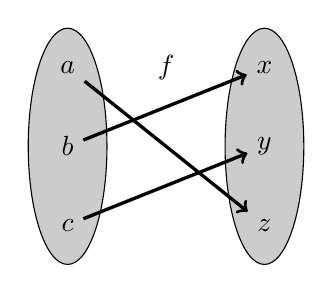
\begin{tikzpicture}[scale=0.5]
        \filldraw (1,3)[fill=black!20!white] circle [x radius=1cm, y radius=3cm];
        \filldraw (6,3)[fill=black!20!white] circle [x radius=1cm, y radius=3cm];
    
        \draw (3.5,5) node {$f$};
    
        \draw (1,5) node(a) {$a$};
        \draw (1,3) node(b) {$b$};
        \draw (1,1) node(c) {$c$};
    
        \draw (6,5) node(x) {$x$};
        \draw (6,3) node(y) {$y$};
        \draw (6,1) node(z) {$z$};
    
        \draw[->,very thick] (a) -- (z);
        \draw[->,very thick] (b) -- (x);
        \draw[->,very thick] (c) -- (y);
    \end{tikzpicture}
\end{minipage}%
\begin{minipage}{.5\textwidth}
    \centering
    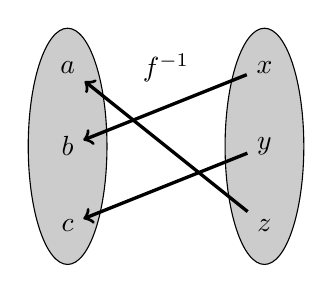
\begin{tikzpicture}[scale=0.5]
        \filldraw (1,3)[fill=black!20!white] circle [x radius=1cm, y radius=3cm];
        \filldraw (6,3)[fill=black!20!white] circle [x radius=1cm, y radius=3cm];
    
        \draw (3.5,5) node {$f^{-1}$};
    
        \draw (1,5) node(a) {$a$};
        \draw (1,3) node(b) {$b$};
        \draw (1,1) node(c) {$c$};
    
        \draw (6,5) node(x) {$x$};
        \draw (6,3) node(y) {$y$};
        \draw (6,1) node(z) {$z$};
    
        \draw[<-,very thick] (a) -- (z);
        \draw[<-,very thick] (b) -- (x);
        \draw[<-,very thick] (c) -- (y);
    \end{tikzpicture}
\end{minipage}

    \caption{A bijective function and its inverse function}
    \label{fig:zermelo_fraenkel_set_theory:bijective_function_and_inverse}
\end{figure}
\begin{proposition}
    A function is bijective if and only if its inverse is a function as well.
\end{proposition}
\begin{proof}
    We will only need to prove one direction of the equivalence because of the total-surjective and univalent-injective dualities. Suppose $f$ is bijective. The domain of $f^{-1}$ is $Y$. By surjectivity of $f$, for any $y\in Y$ there exists an $x\in X$ such that $f(x)=y$, so $(y,x)\in f^{-1}$ and hence $f^{-1}$ is total. Furthermore, this $x$ is unique by injectivity of $f$, and hence $f^{-1}$ is univalent.
\end{proof}

It is often useful to apply one function after the other, so that the output of one function becomes the input of another. We can define this as follows.
\begin{definition}[Function composition]
    Let $f:X\to Y$ and $g:Y\to Z$ be functions. Introduce the binary function symbol $g\circ f$ by
    \begin{equation*}
        g\circ f:=\{(x,z)\in X\times Z\mid\exists y\in Y((x,y)\in f\land(y,z)\in g)\}
    \end{equation*}
    called the composition of $g$ and $f$.
\end{definition}

Lastly we will introduce another useful function symbol. This will allow us to quickly write down the set of functions between any two sets.
\begin{definition}[Set exponentiation]
    We introduce the binary function symbol $Y^X$ by
    \begin{equation*}
        Y^X=\{f\in\mathcal{P}(X\times Y)\mid f:X\to Y\}.
    \end{equation*}
\end{definition}
\end{document}
